\chapter{Basic}

\section{Mechine Learning}
\begin{itemize}
    \item supervised learning
    \item semi-supervised learning
    \item unsupervised learning
    \item reinforcement learning
    \item active learning
    \item transfer learning
\end{itemize}

\section{iid}

\section{Convolution}
\section{Transposed Convolution}
\begin{equation}
    \begin{split}
        H_{out} &= (H_{in} - 1) \times \text{stride}[0] - 2 \times \text{padding}[0] + \text{dilation}[0]
        \times (\text{kernel\_size}[0] - 1) + \text{output\_padding}[0] + 1 \\
    W_{out} &= (W_{in} - 1) \times \text{stride}[1] - 2 \times \text{padding}[1] + \text{dilation}[1]
        \times (\text{kernel\_size}[1] - 1) + \text{output\_padding}[1] + 1
    \end{split}
\end{equation}

\section{Universal approximation theorem}
\begin{quotation}
    Any continuous function can be uniformly approximated by a continuous neural network having only one
    internal, hidden layer and with an arbitrary continuous sigmoidal nonlinearity.\cite{Cybenko1989}
\end{quotation}

万能近似定理最初以sigmoidal激活函数来描述,后被证明对于更广泛的激活函数也适用\cite{Leshno1993},包括ReLU。

\section{Initialization scheme}
\subsection{constant initialization}

\subsection{random initialization}
按照某一分布随机初始化
\subsubsection{normal initialization}
\begin{equation}
    W \sim \N(\mu, \sigma^2)
\end{equation}

\subsubsection{uniform initalization}
\begin{equation}
    W \sim U[-\frac{1}{\sqrt{n}}, \frac{1}{\sqrt{n}}]
\end{equation}

\subsection{xavier initalization}
针对使用\textbf{对称激活函数}$\tanh(x)$的网络进行参数初始化,对于ReLU激活函数并不适用\cite{Glorot2010}.

\subsubsection{Forward}
对于一个卷积层来说
\begin{equation}
    \begin{split}
        y_l &= W_l X_l + b_l\\
        X_l &= f(y_{l-1})
    \end{split}
\end{equation}
在如下前提和假设下
\begin{itemize}
    \item 初始化$W_l$元素为独立同分布
    \item 假设$X_l$元素也为独立同分布
    \item $W_l$, $X_l$互相独立
\end{itemize}
则有
\begin{equation}
    \begin{split}
        Var(y_l) &= Var(\sum W_l X_l + b_l)\\
        &= Var(\sum W_l X_l) \\
        &= n_l Var(W_l X_l)
    \end{split}
\end{equation}
令$W_l$期望为0,$E(W_l) = 0, Var(W_l) = E(W_l - E(W_l))^2 = EW_l^2$,则
\begin{equation}
    \begin{split}
        Var(y_l) &= n_l E(W_l^2X_l^2) - n_l E^2W_l E^2 X_l \\
        &= n_l E(W_l^2X_l^2) \\
        &= n_l Var(W_l)E(X_l^2)
    \end{split}
\end{equation}
若$EX_l = 0$,则
\begin{equation}
    Var(y_l) = n_l Var(W_l)Var(X_l)
\end{equation}

若要实现$Var(y_l) = Var(X_l)$,则需要满足$n_l Var(W_l) = 1$,即
\begin{equation}
    Var(W_l) = \frac{1}{n_l}
\end{equation}

\begin{itemize}
    \item 若$W_l$服从正态分布,则$W_l \sim N(0, \frac{1}{n_l})$
    \item 若$W_l$服从均匀分布,则$W_l \sim U(-\sqrt{\frac{3}{n_l}}, \sqrt{\frac{3}{n_l}})$
\end{itemize}

\subsubsection{Backword}
反向传播过程中,需要保证梯度的方差不变,每一层的梯度为:
\begin{equation}
    \Delta X_l = \hat{W}_l \Delta y_l
\end{equation}
假设
\begin{itemize}
    \item $W_l$和$\Delta{y}_l$互相独立
    \item $EW_l = 0, E\Delta{X}_l = 0$
\end{itemize}
同前向传播,可得
\begin{equation}
    \begin{split}
        Var(\Delta{X_l}) &= \hat n_l Var(W_l)Var(\Delta{y}_l)
    \end{split}
\end{equation}
\begin{itemize}
    \item 若$W_l$服从正态分布, 则$W_l \sim N(0, \frac{1}{\hat n_l})$
    \item 若$W_l$服从均匀分布,则$W_l \sim U(-\sqrt{\frac{3}{\hat n_l}}, \sqrt{\frac{3}{\hat n_l}})$
\end{itemize}

除非$n = \hat n_l$,否则同时保证信号在向前向后传播时的Var不变,取调和平均数,$Var(W_l) = \frac{2}{n_l + \hat n_l}$,可得
\begin{itemize}
    \item Normal distribution: $W_l \sim \N(0, \frac{2}{n_l + \hat n_l})$
    \item Uniform distribution: $W_l \sim \mathcal{U}(-\sqrt{\frac{6}{n_l+\hat n_l}}, \sqrt{\frac{6}{n_l+\hat n_l}})$
\end{itemize}


\subsection{orthogonal initalization}

\subsection{kaiming initalization}
Xavier 针对对称激活函数的层权重初始化进行设计,但对于使用ReLu激活函数的层并不适用\cite{He2015}。
-> 期望为0, 方差为1
\par
对ReLU层来说,$E(X_l^2) = \frac{1}{2}Var(y_l)$,因此
\begin{equation}
    \begin{split}
        Var(y_l) &= \frac{1}{2} n_l Var(W_l)Var(X_l) \\
        Var(\Delta{X_l}) &= \frac{1}{2} \hat n_l Var(W_l)Var(\Delta{y}_l)
    \end{split}
\end{equation}
且在权重初始化时,使用上述任意一个即可。

\section{Regularization}

\section{Data proprocessing}
\subsection{whitening}

\section{Activation functions}
\subsection{sigmoid}
\begin{tikzpicture}[domain=-2:2]
    \draw[very thin,color=gray] (-1.9, -1.9) grid (1.9, 1.9);
    \draw[->] (-2,0) -- (2,0) node[right] {$x$};
    \draw[->] (0,-2) -- (0,2) node[above] {$f(x)$};
    \draw[color=red]	plot (\x, { 1 / (1 + exp(-3*\x)) })   	node[right] {$g(x) = \frac{1}{1 + \mathrm{e^{-x}}}$};
\end{tikzpicture}

\begin{equation}
    \begin{split}
        g(x) &= \frac{1}{1+\mathrm{e}^{-x}} \\
        g(x)' &= g(x)(1-g(x))
    \end{split}
\end{equation}

\subsection{tanh(x)}
\begin{tikzpicture}[domain=-2:2]
    \draw[very thin,color=gray] (-1.9, -1.9) grid (1.9, 1.9);
    \draw[->] (-2,0) -- (2,0) node[right] {$x$};
    \draw[->] (0,-2) -- (0,2) node[above] {$f(x)$};
    \draw[color=blue]	plot (\x,{tanh(\x)})					node[right] {$g(x) = \tanh(x)$};
\end{tikzpicture}

\begin{equation}
    \begin{split}
        g(x) &= tanh(x) \\
        g(x)' &= 1 - g(x)^2 \\ &= 1 - \tanh(x)^2
    \end{split}
\end{equation}

\subsection{Rectified linear units}
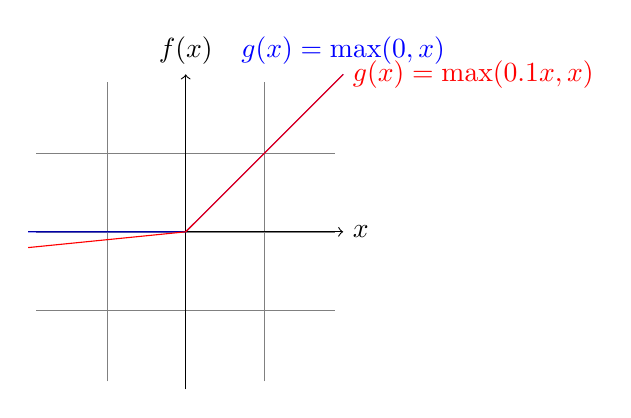
\begin{tikzpicture}[domain=-2:2]
    \draw[very thin,color=gray] (-1.9, -1.9) grid (1.9, 1.9);
    \draw[->] (-2,0) -- (2,0) node[right] {$x$};
    \draw[->] (0,-2) -- (0,2) node[above] {$f(x)$};
    \draw[color=blue]	plot (\x,{max(0, \x)})					node[above] {$g(x) = \max(0, x)$};
    \draw[color=red]	plot (\x,{max(0.1 * \x, \x)})			node[right] {$g(x) = \max(0.1x, x)$};
\end{tikzpicture}



\begin{table}[h]
	\centering
	\small
	% \resizebox{\linewidth}{!}{
		\begin{tabular}{c|c|c|c}
			\toprule
			Name            & Plot 	        & $f(x)$   & $f'(x)$    \\
			\midrule
			Sigmoid  		&   		    & $\sigma(x) = \frac{1}{e^{-x} + 1}$ & $\sigma(x)(1-\sigma(x))$\\
            \normalrule
            Tanh            &               & $\tanh(x) = \frac{e^x-e^{-x}}{e^x+e^{-x}}$    & $1 - \tanh(x) ^ 2$\\
            \normalrule
            ReLU            &               & $\max(0, x)   $   & \\
            \normalrule
            Leaky ReLU      &               & $\max(0.01x, x)$  & \\
            \normalrule
            PReLU           &               & $\max(\alpha x, x)$ & \\
            \normalrule
            SiLU/Swish      &               & $x \sigmoid(x) = \frac{x}{e^{-x} + 1}$    & \\
            \normalrule
            Mish            &               & $x\tanh(\ln(1+e^{x}))$ & \\
            \normalrule
            ELU             &               & $\begin{cases}
                \alpha(e^x - 1) & x \leqslant 0\\
                x               & x > 0
            \end{cases}$  &$ \begin{cases}
                \alpha e^x & x \leqslant 0 \\
                1          & x > 0
            \end{cases}$\\
            \normalrule
            SELU            &               & \makecell{$\lambda \begin{cases}
                \alpha(e^x - 1) & x < 0\\
                x               & x \geqslant 0
            \end{cases}$ \\
            $\lambda = 1.0507, \alpha = 1.67326$}
             & $\lambda \begin{cases}
                 \alpha e^x & x < 0 \\
                 1          & x \geqslant 0
            \end{cases}$\\
            \normalrule
            Softplus        &               & $\ln(1 + e^x)$ & $\sigma(x) = \frac{1}{e^{-x} + 1}$\\
			\bottomrule
	    \end{tabular}
	% }
	\caption{Activation functions}
	\label{tab:activation_functions}
\end{table}

\subsection{Loss functions}
深度学习基本使用最大似然估计进行训练,因此代价函数就是\textbf{负的对数似然}(The negative log likelihood loss),他与训练数据和模型分布间的
交叉熵等价
\[
    J(\theta) = - \E_{\vx, \vy \sim P} \log Q(\vy|\vx)
\]
代价函数的具体形式依赖于$\log Q(\vy|\vy)$的具体形式

\subsubsection{Autoencoder重构误差}
\begin{align}
    Q(\vy|\vx)  &= \N(\vy; f(\vx; \theta), \mI) \\
    J(\theta)   &= -\E_{\vx, \vy \sim P} \log ( \frac{1}{\sqrt{2 \pi}} e ^{-\frac{(\vy - f(\vx; \theta))^2}{2}}) \\
                &= -\E_{\vx, \vy \sim P} (-\frac{(\vy - f(\vx; \theta))^2}{2}) + constant \\
                &= \frac{1}{2} \E_{\vx, \vy \sim P} (\vy - f(\vx; \theta))^2 + constant \\
                &= \frac{1}{2} \E_{\vx, \vy \sim P} \|\vy - f(\vx; \theta)\|^2 + constant
\end{align}



\section{Batch Normalization}
机器学习中假设:源空间和目标空间的数据分布是一致的,如果不一致,就是新的机器学习问题,例如transfer learning/domain adaptation
等。而covariate shift就是分布不一致假设下的一个分支问题,它指的是源空间和目标空间的条件概率是一致的,但是其边缘概率不同.
对于所有$x \in \chi $
\begin{equation}
    \begin{split}
        P_s(Y|X = x) &= P_t(Y|X = x) \\
        P_s(X) &\neq P_t(X)
    \end{split}
\end{equation}
\begin{quotation}
    \textbf{Internal Covariate Shift} Training Deep Neural Networks is complicated by the fact that the distribution of each layer's inputs
changes during training, as the parameters of the previous layers change. And this slows down the training
by requring lower lr ant careful parameter initialization, and makes it notoriously hard to train models
with saturating nonlinearities.
\end{quotation}
解决方案:白化操作可以使得数据变为\textbf{独立同分布}
\begin{quotation}
    By whitening the inputs to each layer, we would take a step towards achieving the fixed distribution
    of inputs that would remove the ill effects of the ICS.
\end{quotation}
但是每层的白化会影响梯度下降优化过程。每层进行白化计算量过大。保证模型的表达能力不因为规范化而下降。

Simply normalizaing each input of a layer may change what the layer can represent. So, we make sure that
the transformation inserted in the network can represent the identity transform.
\begin{figure}[H]
    \centering
    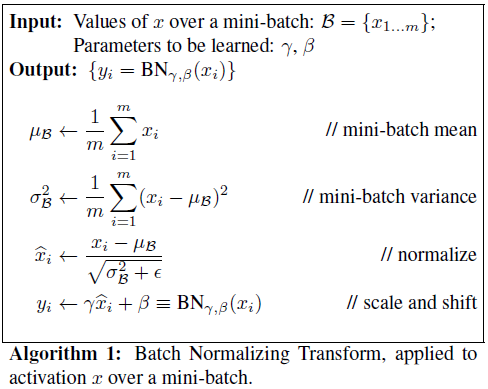
\includegraphics[width=8.5cm]{images/bn_algorithm.png}
    \caption{Batch Normalization}
    \label{fig:batchnorm}
\end{figure}

\section{How Does Batch Normalization Help Optimization?}
Batch Normalization 对减少ICS起到了很少的作用,it makes the optimization landscape significantly smoother.
\begin{itemize}
    \item \textbf{Is the effectiveness of BatchNorm indeed related to internal covariate shift?} The 'noisy' BatchNorm
    network has qualitatively less stable distributions than even the standard, non-BatchNoram network, yet it still
    better performs better in terms of training.
    \item \textbf{Is BatchNorm reducing internal covariate shift?} We Observe that networks with BatchNorm often
    exhibit an increase in ICS.
\end{itemize}
\begin{figure}[H]
    \centering
    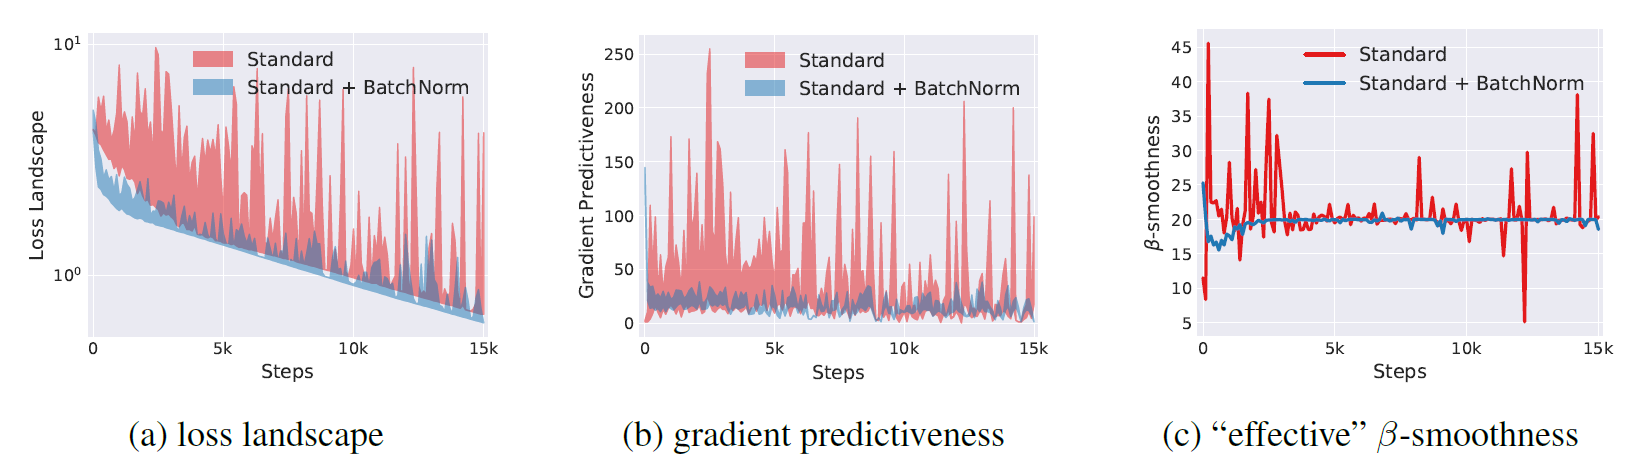
\includegraphics[width=14cm]{images/bn_landscape.png}
    \label{fig:bn_landscape}
\end{figure}

\textbf{Why does BatchNorm work?}


BatchNorm reparametrizes the underlying optimization problem to make its landscape significatly more smooth.
The key implication of BatchNorm's reparametrization is that it makes the gradients more reliable and predictive.
After all, improved Lipschitzness of the gradients gives us confidence that when we take a larger step in a direction
of a computed gradient, this gradient direction remains a fairly accurate estimate of the actual gradient direction after
taking that step.

\textbf{Is BatchNorm the best way to smoothen the landscape?}

In fact, for deep linear networks, $l_1$–normalization performs even better than BatchNorm. Note that,
qualitatively, the $l_p$–normalization techniques lead to larger distributional shift than the vanilla,
 i.e., unnormalized, networks, yet they still yield improved optimization performance.
